\documentclass{acm_proc_article-sp}
\newcommand\floor[1]{\lfloor#1\rfloor}
\newcommand\ceil[1]{\lceil#1\rceil}
\newcommand{\tabitem}{~~\llap{\textbullet}~~}
\usepackage{textcomp}
\usepackage{url}
\usepackage{algorithm}% http://ctan.org/pkg/algorithms
\usepackage[noend]{algpseudocode}
\usepackage{pifont}
\usepackage{tabulary}
\usepackage{amsmath}
\usepackage{float}
\usepackage{cleveref}
\usepackage{caption}
\DeclareCaptionType{copyrightbox}
\usepackage{subcaption}
\usepackage{pgfplots}
\usepackage{graphicx}
\usepackage{subfig}
\usepackage{tabularx}
\usepackage{capt-of}
\usepackage[utf8]{inputenc}
\DeclareMathOperator*{\argmax}{argmax}
\newcommand*{\argmaxl}{\argmax\limits}
\newcommand{\norm}[1]{\left\lVert #1 \right\rVert}
\usepackage{eqparbox}
\renewcommand{\algorithmiccomment}[1]{\hfill\eqparbox{COMMENT}{ \textit{\small{\hspace{0.5cm}//#1}}}}

\begin{document}
\title{Who to query? \\DispNN: A two-stage querying algorithm for identifying events with variant/unknown spatial distributions }
\numberofauthors{3} %  in this sample file, there are a *total*
\author{
% You can go ahead and credit any number of authors here,
% e.g. one 'row of three' or two rows (consisting of one row of three
% and the second row of one, two or three).
%
% The command \alignauthor (no curly braces needed) should
% precede each author name, affiliation/snail-mail address and
% e-mail address. Additionally, tag each line of
% affiliation/address with \affaddr, and tag the
% e-mail address with \email.
%
% 1st. author
\alignauthor
Mai ElSherief\\
 \affaddr{Dept. of Computer Science }\\
 \affaddr{UC Santa Barbara}\\
%\affaddr{Santa Barbara, CA}\\
 \email{mayelsherif@cs.ucsb.edu} 
 \alignauthor
Ramya Raghavendra\\
 \affaddr{IBM T. J. Watson Research Center }\\
 \email{rraghav@us.ibm.com}
% 2nd. author
\alignauthor
Elizabeth Belding\\
\affaddr{Dept. of Computer Science }\\
 \affaddr{UC Santa Barbara}\\
 %\affaddr{Santa Barbara, CA}\\
 \email{ebelding@cs.ucsb.edu}
}
\maketitle
\begin{abstract}
The ubiquity of sensors, whether devices or humans, and the resulting explosion of critical applications have resulted in 
the need to address a variety of new opportunities and challenges. In this paper, we propose DispNN: a two-stage node selection algorithm for resource constrained systems based on node locations to identify incidents in a $2D$ spatial environment. Given a constraint of $N$ probes, DispNN uses a subset of $N$ to probe nodes that maximize the dispersion of node locations. Based on the response received from the queried nodes, DispNN then probes the K nearest neighbors using the rest of the available $N$ probes. We evaluate DispNN algorithm on three different distributions: clustered, uniform and long-tailed. We then apply the algorithm to a dataset of street harassment provided by Hollaback. The proposed algorithm outperforms a random selection approach by up to $63\%$ and an approach of dispersion maximization by up to $68\%$.
\end{abstract}
%\category{H.1.2}{User/Machine Systems}{Human information processing}
%\keywords{Street harassment, Urban analysis, Walkability score, Transit Score, Transit route }
\section{Introduction}
Sensors have become an integral part of daily life. The common smartphone includes a variety of different sensors, such as camera, microphone, GPS, accelerometer, digital compass, light sensor, and Bluetooth as a proximity sensor. The ubiquity of sensors is also prevalent in the urban environment. Examples include traffic sensors, agriculture sensors, wireless parking sensors, infrastructure sensors, weather, and pollution sensors. Data analysis from such sensors yield important observations. For instance, ~\cite{ferreira2013visual} leverages the geographic and temporal data associated with taxis in NYC to gain insight into multiple aspects of city life, from economic activity and human behavior to mobility patterns. When combined with crowdsourcing of human input, critical environmental data can be generated. One example is the application ``Waze'', where users can report traffic jams, accidents and other road related incidents in real-time. The work in~\cite{agapie2015crowdsourcing} uses local workers to collect data at different events, that were mostly open to the public (e.g. a neighborhood fest, an art show, a music festival and others), and remote workers to curate the collected information and generate event reports.\par

One of the most pressing challenges of sensor ubiquity is energy preservation. All systems are bound by a fixed amount of resources; sensor nodes are typically the most constrained. For instance,~\cite{marco2003many} and~\cite{pattem2008impact} focus on eliminating redundancies among correlated sensor measurements. In this paper, we investigate the problem of how we can probe a limited subset of sensors in a particular environment in order to preserve energy or other resources. Examples of resource constrained systems include disaster and safety applications. In an emergency, communication networks tend to fail and available resources, such as bandwidth, are scarce~\cite{manoj2007communication}.\par


In particular, we envision a scenario where users/sensors can be probed to collectively answer some question. An unanswered question can be related to a phenomenon that needs to be identified under the constraints of $N$ resources. In~\cite{crooks2013earthquake}, the unanswered question was related to if users felt a 5.8 magnitude earthquake which occurred on the East Coast of the United States (US) on August 23, 2011. The experiments in this work, analyzing the spatial and temporal characteristics of the twitter feed activity support the notion that people act as sensors to give us comparable results in a timely manner. In this scenario, our algorithm can be used to query human resources in the geographic area affected by the earthquake. The earthquake can affect network performance and impose a resource constraint on the number of people queried. Another example of safety applications is what happens in Tahrir Square during Egyptian revolutions in 2011 and 2012. At that time, women were discouraged from participation due to the high harassment rates~\cite{guardianSH}. This resulted in movements of men forming protective human shields~\cite{worldPostHS} around female protestors to avoid assault. In this scenario the unasnwered question would be ``Is it safe in your location?'' or ``Is it harassment free in your location?''. The resource constraints in this scenario would arise from avoiding disturbing the millions of people in the sqaure and avoiding the base stations overload in this area.  
Our proposed algorithm can be used to query users for safe zones for women and then use the results for safe routing around the square or for identifying zones where women can safely participate in the protests. \par


In this paper we introduce DispNN (Dispersion-Nearest Neighbors): a generic two-stage querying/probing algorithm that aims to maximize the \textit{dispersion} of nodes locations in the first stage and then in the second stage, it selects the \textit{nearest neighbors} for nodes that provide a positive feedback about incidents in their surroundings. Our contribution in this paper is three-fold. First, we propose DispNN: a two-stage matching algorithm that attempts to gain information about incidents when there is no prior information about the spatial distribution while conserving resources.  Secondly, we study the performance of our proposed algorithm under three different distributions: clustered, uniform and long-tailed. The initial algorithm outperforms the random user selection by up to $63\%$ in terms of selecting nodes that are closer (in the K nearest neighbors (KNN) sense) to the events and outperforms the dispersion maximization algorithm by up to $68\%$. We then test the algorithm on a real dataset of street harassment reports in different cities and show the applicability of using DispNN in detecting incidents and in locating users close to these incidents. Third, we discuss how the algorithm can be modified in the case of untrustworthy nodes based on trust variations or prior knowledge availability of the spatial distribution.\par
The rest of this paper is organized as follows. Section 2 surveys the related work while Section 3 describes DispNN. Section 4 experimentally evaluates DispNN, and Section 5 discusses tradeoffs and variations of DispNN. Section 6 concludes the paper.
\section{Related Work}
Since the introduction of ``crowdsourcing'' as a modern business term in 2006~\cite{howe2006rise}, a significant body of work has been dedicated to the study and implementation of crowdsourcing in real life applications. In particular, spatial crowdsourcing, where crowd participation is bound to a particular geographic area, has received significant attention~\cite{kazemi2012geocrowd, deng2013maximizing, yu2015quality}. For instance, ~\cite{liu2013using} introduces a location-based real-time social question answering service, where users can ask temporal and geo-sensitive questions and then receive answers that are crowdsourced in a timely fashion. A crowdsensing platform was introduced in~\cite{cardone2013fostering} to facilitate the collaboration of large groups of people participating in collective actions of urban crowdsourcing. Our work is different in the sense that it imposes a constraint on the number of nodes who can be queried in order to conserve resources. This is particularly important to avoid disturbing a large number of people in a crowded geographic area, such as a concert or protest. In addition, this prevents the querying server from entering a state of response overload.\par

Using people as sensors, collective sensing, and citizen science have opened doors for interesting research problems. Some of these challenges are introduced in~\cite{blaschke2011collective}. One important challenge in geo-crowd sensing is detecting unusual events. The work proposed in~\cite{lee2010measuring} leverages microblogging websites such as Twitter to detect unusual geo-social events by identifying unusually crowded regions. Another challenge is the refinement of crowd sensed data and detection of fake data. Solutions based on a user's history and reputation have been introduced in the literature. The work in~\cite{yu2013reputation} proposes a reputation-aware model that balances the workload between users. Another challenge is fusing untrustworthy estimates~\cite{venanzi2013trust}. Taking into account spatial properties, ~\cite{venanzi2013crowdsourcing} tackles the problem of merging multiple spatial observations reported by possibly untrustworthy users using a heteroskedastic Gaussian process model. In this paper, as opposed to detecting unusual events~\cite{blaschke2011collective}, we provide a generic framework to answer a pre-specified question by querying a subset of sensors, whether human or devices, in the spatial area. Detecting untrusted responses is not the main focus of our paper. Instead, we assume that a trust algorithm can be built on top of our algorithm to eliminate untrusted responses.\par

Another related body of work is sensor networks~\cite{akyildiz2002survey} that include spatially and ubiquitously distributed autonomous sensors used to monitor physical and environmental conditions. Since the sensors are typically small, low-powered nodes, resource-constrained protocols emerged to preserve the energy of these devices. Examples of work targeting energy preservation include, but are not limited to~\cite{sallai2004acoustic}, where the authors achieve geographic localization using a noise tolerant acoustic ranging mechanism to meet severe resource constraints. In~\cite{krishnamachari2002impact}, data aggregation methods were introduced and achieved significant performance gains in comparison to end to end routing. The work proposed in~\cite{fontugne2013strip} implements a system that analyzes sensor behaviors and uncovers misbehavior corresponding to inefficient device usage that leads to energy waste. In contrast, our work focuses on the how to choose sensors to query based on their location while constraining the number of probes to a subset of the total number of sensors hence, preserving energy.



\section{DispNN: a two-stage querying algorithm}
In our system, we have a two-dimensional grid and a number of objects that can sense the environment around them. These objects can be humans, artificial sensors, mobile phones or even robotic sensors. We are interested in answering questions of the form: ``What is the answer to Question X in this grid?". For instance a question can be ``Is it safe around you?'', or `` Did you feel the earthquake?''. To find the answer, one approach would be to query all the objects in the two-dimensional space and aggregate the findings. However, in many situations, such as during emergencies or in long term sensor deployements preserving resources such as energy is critical~\cite{manoj2007communication}. In this paper, we investigate how to answer the aforementioned question in the case of limited resources. Hence, the question becomes: \textit{Given $M$ nodes and $N$ resources, where $N < M$, which $N$ nodes should be queried to obtain the needed answer?}\par


If we tackle this question from a probabilistic point of view, then the straightforward answer is to try to select objects with the same probabilistic distribution as the phenomenon. For instance, if we know that a certain phenomenon occurs uniformly in the two-dimensional grid, then we would have no bias in selecting the users to query, i.e. each user/object should have the same probability of selection to be queried. On the other hand, if we know the phenomenon we are interested in is more prevalent in certain areas of the grid as opposed to other areas, we should take that into consideration when we are selecting the nodes such that we query devices in the area of interest and fewer devices in areas where there is a smaller probability of occurrence.\par

The question becomes far more challenging if the distribution is not known or if it is time variant. In this case, we inquire if there is a systematic algorithm that can be used for querying/selecting users to spatially identify a phenomenon regardless of the probabilistic distribution or time variation. In the following sections, we describe DispNN: a two-stage algorithm that queries objects without any assumptions about the distribution of events and succeeds in locating nodes that are close to the events and in covering up to approximately $90\%$ of the incidents. \par

\subsection{Algorithm description}
We assume that there are $M$ users in a two-dimensional grid and that the system that selects a user to query is bounded by $N$ resources, where $N < M$.  Each of the $M$ users has a specific location in the grid, determined by a two-dimensional system, e.g. (x, y) or a (lat, long). We also assume that the selected devices will fully cooperate and respond to the query. If needed, a pre-selection phase can be used to eliminate users that are not likely to co-operate, such as requiring the installation of an app to facilitate querying. Here, we focus on how to select $N$ out of $M$ users, where $N < M$, to identify both events occurring in the two-dimensional grid and nodes that are close to these events.\par

Given $N$ nodes, DispNN divides the selection of nodes into two stages as depicted in Algorithm~\ref{TSalgorithm}. The number of queried devices in the first stage is determined by $\floor{(FSP*N)}$ where FSP denotes the first stage percentage. As indicated in Table~\ref{table:systemParameters}, the first stage percentage represents the fraction of nodes that will be selected to be queried in the first stage of DispNN. In the first stage, our goal is to select nodes that maximize the dispersion of their locations. This is accomplished by selecting the set of points, $\mathcal{P} = \{ p(i), \ i \in \{ 1,..., \floor{(FSP*N)} \}$, that maximize the average distance between each point and its nearest neighbor as follows:
\begin{equation} \label{eq:maxDisp}
\argmax\limits_{\mathcal{P}} \sum_{i=1}^{|\mathcal{P} |} \norm{p(i) - NN(p(i))}^2
\end{equation}


\begin{algorithm}[!htb]
\caption{DispNN querying algorithm}
\label{TSalgorithm}
\begin{algorithmic}[1]
   \Function{selectUsersFromGrid }{$FSP, N$}
       \State selectedUsers = $\left\{\right\}$
       \State firstStageCnt = $\floor{(FSP*N)}$
       \State secondStageCnt = M - firstStageCnt
        \Comment{First Stage: Maximize dispersion with firstStageCnt}
       \State firstStageUsers = maximizeDisp(firstStageCnt) 
       \State usersFeedback = feedback(firstStageUsers)
       \Comment{(a) Identify pivot nodes}
        \If {usersFeedback.size == 0} 
         \Comment{Second Stage:}  
              \State selectedUsers = maximizeDisp(secondStageCnt){}
       \Else
           \State {selectedUsers.append(firstStageUsers)}
       \EndIf    
     \State firstStageQuota = calculateQuota(firstStageUsers)  \Comment{(b) Get NNs for pivot users depending on quota}
     \Comment{or maximize dispersion}
     \For{$user_i$ in firstStageUsers}
   \State selectedUsers.append(KNN($user_i$, $firstStageQuota_i$))  \Comment{Aggregate selected users}
 \EndFor
\State return {selectedUsers}
\EndFunction
\end{algorithmic}
\end{algorithm}


where $p$ represents a point in the $2D$ grid and $NN$ represents the nearest neighbor; the distance is measured as the Euclidean distance. The algorithm attempts to maximize the dispersion with a percentage of the $N$ resources up a certain number of trials controlled by the ``maximization trials'' setting, as defined in Table~\ref{table:systemParameters}. \par
After the first stage of dispersion maximization, stage 2 consists of querying the sensors that were selected and evaluating the response of these sensors. The response provided is application dependent. For some applications, the query can be in the form of probing for some measurement and if that measurement exceeds a certain threshold, the system marks this as a positive response to the incident under investigation. In other applications, the query could be a simple yes-no question. An example is in~\cite{crooks2013earthquake}, when an earthquake occurred on the East Coast in the US in 2011, the query was the question ``Did You Feel It?''.\par

 Based on the node response in the first stage, we then proceed to a more fine-grained selection. The objects that provide a positive response, where the definition of a positive response is application dependent, are called the \textit{pivot users}. After response inspection, we divide the rest of the resources ($N-\floor{FSP*N}$) among the nearest neighbors for each of the pivot users. If no nodes provide a positive response, the second stage maximizes the dispersion of the location of nodes with the rest of the available resources. In our analysis, we test the cases of setting $FSP = 20\%, 40\%, 60\%$ and $80\%$ of the $N$ resources in the first stage. \par

This initial algorithm assumes that the first stage nodes will respond with unfalsified responses. To relax this assumption, we explore dividing the selection of the second stage users into two groups: a group that consists of the $KNN$ of trusted pivot users, and another group that aims to maximize the dispersion. In the next section, we focus on studying DispNN with the assumption of having full trust in the crowd and discuss other variants of the algorithm in Section 5.\par

\begin{table}{}
\centering
\begin{tabulary}{0.5\textwidth}{|L|}
\hline
\textbf{Environment settings:}\\
\tabitem \textit{matrix dimension:} the length and width of the $2D$ spatial matrix. We model the spatial area under investigation as a $2D$ square matrix.\\
\tabitem \textit{incident count:} number of incidents distributed across the cells of the spatial matrix\\
\tabitem \textit{resources or crowd count:} the $M$ resources from which $N$ will be chosen to query, where $N < M$.\\
\hline
\textbf{Query settings:}\\
\tabitem \textit{$N$:} the number of resources the system is limited by to query/sense \\
\tabitem \textit{first stage percentage (FSP):} the percentage of users/sensors of the $N$ resources that will be selected to query in the first stage.\\
\tabitem\textit{$k$:} used to identify the KNN crowd individuals/sensors to an incident\\
\hline
\textbf{Approximation settings: }\\
\tabitem \textit{maximization trials:} number of attempts to maximize the dispersion of selected individuals/sensors from the crowd\\
\hline
\end{tabulary}
\caption{Parameters of DispNN.}
\label{table:systemParameters}
\end{table}

\section{Experiments}
To quantify the performance of our algorithm, we perform multiple experiments with three types of data spread: clustered, uniform and real datasets. In our experiments, we compare our algorithm in the selection of users to two alternative approaches as follows:
\begin{itemize}
\item Random user selection: For this approach, we select $N$ users randomly based on a uniform distribution.
\item Dispersion maximization (DispMax) selection: In this approach, $N$ users are selected from the resources/crowd who maximize the dispersion of their locations.
\end{itemize}

\subsection{Experiment variables}
There are multiple variables that can be controlled to test the behavior of DispNN. Table~\ref{table:systemParameters} summarizes the most important.
The environment settings are related to the size of the $2D$ matrix, the number of incidents, the distribution of incidents across the matrix, and the number of resources from which to choose. In all of our experiments, except the case study, we set up the $2D$ matrix as a $10$ by $10$ matrix. We show results for incident count of $50$ and number of resources ($M$) of $100$.
We varied the environment settings in our experiments and we do not observe any differences in performance. Instead, we focus on varying the query settings to better understand DispNN. In this section, we vary the first stage percentage and leave the variation of the $k$ setting to the following section. We also show results for $N = 30$, which constitutes $30\%$ of the available resources ($M$). We notice that the gap between the performance of our algorithm and the other approaches increases when $N$ decreases, and all the approaches converge in performance when $N$ approaches $M$. \par

We compare the performance of our algorithm to two alternative selection approaches: random selection and dispersion maximization. To do so, we utilize two different metrics: count of nodes queried in the $KNN$ of incidents, and the number of incidents covered by the nodes queried. For $i \in \{1, ...,\mathcal{I}\}$, let $KNN_i$ be the $KNN$ of the $i$th incident, where $\mathcal{I}$ denotes the total number of incidents. The two metrics are defined as:
\begin{itemize}
\item Close node count (CNC): the absolute number of sensors/resources in the KNN of each incident for all incidents. This is formally represented as follows:
\begin{equation}
Close\ node\ count = \sum\limits_{ i = 1}^\mathcal{I}\ |(KNN_i \cap {QU})|
\end{equation}
where $QU$ (the ``Queried Users'' set) is the set of users selected for querying.
\item Coverage: the number of incidents covered out of the total number of incidents occurring in the $2D$ matrix. We define an incident as covered if at least one of the nodes in the incident's KNN was queried. This is formally measured as:
\begin{equation}
Coverage =  \sum\limits_{ i = 1}^\mathcal{I}\ Coverage_i\  where,
\end{equation}
\[
Coverage_i =
\begin{cases}
1,& \text{if }(KNN_i \cap {QU}) \neq \phi\\
0,              & \text{otherwise}
\end{cases}
\]
\end{itemize}

In our experiments, we simulate the positive response. A node will provide a positive response if it is in the kNN of one or more incidents in the grid. Choosing a small value of $k$ simulates a fine-grained phenomenon like street harassment. In contrast, a large value of $k$ simulates a phenomenon with a larger range like an earthquake. 
%The positive response does not contain any information about the number or location of incidents. The response simply indicates that the person/sensor detected one or more incidents in their range. 
\subsection{Clustered data experiments}
Geographer Waldo R. Tobler's stated in the first law of geography: ``Everything is related to everything else, but near things are more related than distant things.'' In this subsection, we assume that the incidents are related to each other in a clustered way, i.e. they form clusters across the $2D$ spatial matrix as seen in Fig~\ref{fig: clust}. Our goal in this section is to study the performance of the different approaches when the events are clustered.\par
\begin{figure}[!h]
\centering
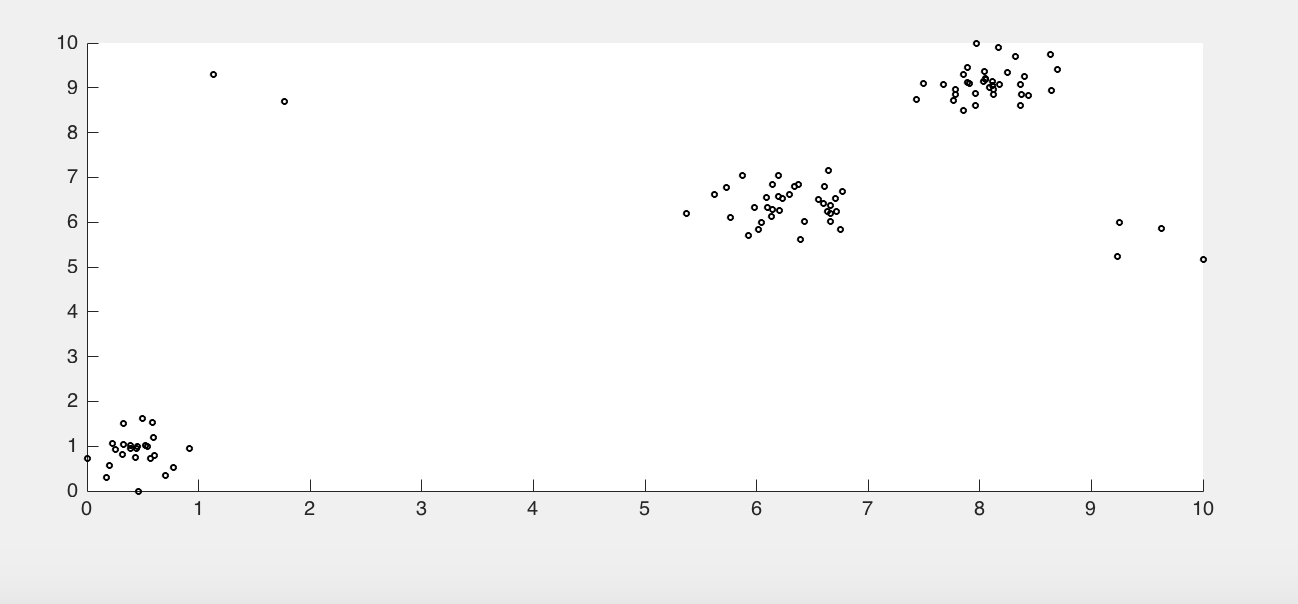
\includegraphics[width=9cm ,height=5.5cm]{figuresPng/clust.png}
\caption{An example of a $2D$ spatial matrix with $5$ clusters.}\label{fig: clust}
\end{figure}

For this set of experiments, we vary the number of clusters in our $2D$ matrix from one to ten clusters while fixing the resources or crowd count to be $100$. To enforce data variability, we model the size of each cluster as a random variable while ensuring that the aggregated size of all the clusters is equal to the crowd count. For each case of number of clusters, we average over $100$ different configurations. Our objective is to measure the effect of variation of the first stage percentage on our performance metrics.\par

Figure~\ref{fig:clusteredResults} depicts the results for CNC when varying the first stage percentage (FSP) from $20\%$ to $80\%$. DispNN always outperforms the Random node selection and the Dispersion Maximization selection. Table~\ref{table:clusteredSurge} depicts the performance gain for CNC in comparison to the Random and Dispersion maximization approaches. As the amount of resources queried in the first stage decreases, CNC increases. This is due to the fact that when the first stage percentage decreases, the second stage resources increase under limited resources constraints, which focuses on resources close to incidents detected in the first stage. On the other hand, incident coverage tends to increase as the first stage count increases. This is depicted in Figure~\ref{fig: clustCoverage}. Both CNC and Incident coverage tend to increase with the number of clusters until the number of clusters is around four or five. Then, they decrease. The reason is that as the number of clusters increases in the grid, so does the probability of success of the first stage in identifying more incidents. On the other hand, as the number of clusters increase, the cluster size decreases which results in fewer incidents per cluster.

%Real life examples of clustered events include
%- Begin by pointing out real-life examples of spatially clustered phenomenon and spatial correlation in general. Lots of social phenomena are spatially dependent. %(https://books.google.com/books?id=jbFRojt85TUC&pg=PA2&lpg=PA2&dq=clustered+phenomena&source=bl&ots=yftMfShveB&sig=XcPOJriI1gineu-%A2YGpoJT3OII&hl=en&sa=X&ved=0ahUKEwiBp4a-s-zKAhUI5WMKHZQ3Cd8Q6AEITzAI#v=onepage&q=clustered%20phenomena&f=false)




%\caption{Average number of nodes close to the incidents (Close node count) as FSP varies.}
%\label{fig:clusteredResults}
\begin{table*}[t]
 \centering
 \begin{tabular}{cc}
    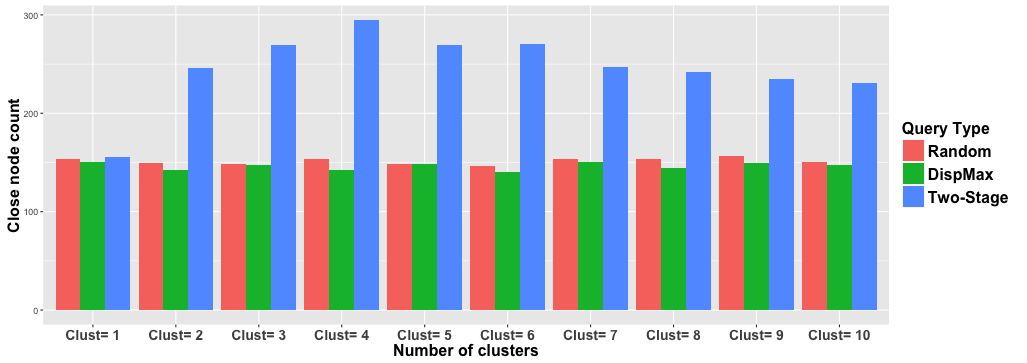
\includegraphics[width=0.5\textwidth]{figuresPng/fsTwentyPerc.png} &  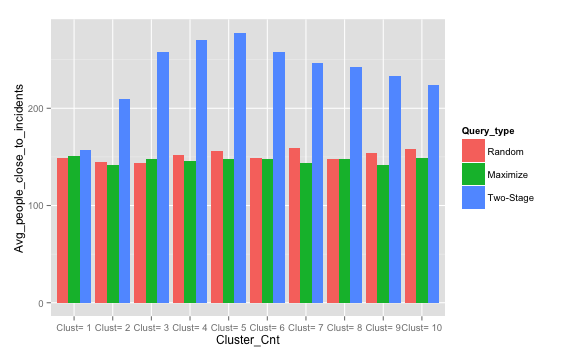
\includegraphics[width=0.5\textwidth]{figuresPng/fsFourtyPerc.png}\\
    (a) Close node count with $FSP = 20\%$ of available resources. & (b) Close node count with $FSP = 40\%$ of available resources.\\
    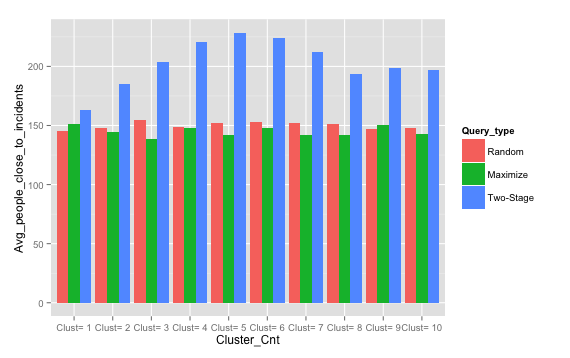
\includegraphics[width=0.5\textwidth]{figuresPng/fsSixtyPerc.png} &  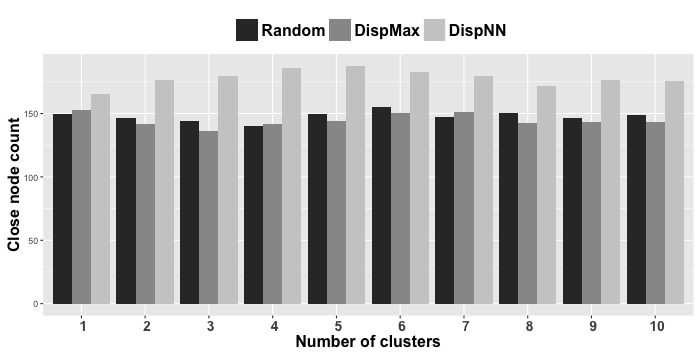
\includegraphics[width=0.5\textwidth]{figuresPng/fsEightyPerc.png}\\
      (c) Close node count with $FSP = 60\%$ of available resources. & (d) Close node count with $FSP = 80\%$ of available resources.\\
 \end{tabular}
  \captionof{figure}{Average number of nodes close to the incidents (Close node count) as FSP varies}
\label{fig:clusteredResults}
\end{table*}

\subsection{Uniformly distributed data experiments}
In the next set of experiments, the probability of occurrence of incidents is uniform across the grid, i.e. $P_I (j) = P_I (k)$ where $j \neq k$ and $P_I$ denotes the probability of an incident occurring at a specific cell. We randomly generate $100$ different matrices and average the results. We note that if we know that the distribution of the incidents is uniform, the best we can do is to choose $N$ nodes uniformly. Using DispNN, we select $N$ nodes without assuming any distribution about the incidents and check the performance in comparison to the uniform random selection, which yields the best results in terms of CNC. Figure~\ref{fig:uniClosePeople} shows that DispNN with $FSP = 20\%$ achieves the highest number of CNC while Figure~\ref{fig:uniIncdCove} shows that DispNN with $FSP = 80\%$ achieves higher coverage that the uniform random policy and it is close to the maximum coverage by an average of $1.32$ incidents. This shows that our algorithm can achieve better node selection than the uniform scheme in terms of close node count when $FSP = 20\%$ and achieves better coverage than the uniform scheme in $FSP = 80\%$.




\subsection{Long tail distribution}
In this subsection, the incidents are generated according to a special case of the Long Tail distribution called the ``Pareto principle''. According to the Pareto principle, we assume that $20\%$ of the matrix cells are home for $80\%$ of the incidents while conversely $80\%$ of the matrix cells are home for $20\%$ of the incidents. We generate $100$ different matrices applying the Pareto Principle randomly on the cells. We use a random uniform distribution to select $20\%$ of the cells and generate $80\%$ of the incidents uniformly for these cells and vice versa. Figure~\ref{fig:LTClosePeople} shows that DispNN outperforms both the random policy and the dispersion maximization policy by up to $10.2\%$ and $12.1\%$, respectively, in terms of CNC. This is due to the clustering of events in only $20\%$ of the grid which means that more than one incident is likely to occur in the same cell. So, if DispNN reaches a node close to an incident in one cell, this same node will cover more than one incident in the same cell. Dispersion maximization achieves the best incident coverage as shown in Figure~\ref{fig:LTIncdCove}. DispNN approaches the maximum incident coverage when $FSP = 80\%$ with a difference of $1.24$ incidents on average. This shows that DispNN with $FSP = 80\%$ can still achieve a balance between CNC and incident coverage.

\begin{table}[!h]
\centering
\begin{tabulary}{0.5\textwidth}{|C|C|C|C|C|}
\hline
First stage percentage & $20\%$ & $40\%$  & $60\%$  & $80\%$  \\ \hline
Performance gain over Random   & $63\%$ & $59\%$  & $35\%$  & $20\%$  \\ \hline
Performance gain over Dispersion Maximization   & $68\%$ & $62\%$  & $40\%$  & $21\%$ \\ \hline
\end{tabulary}
\caption{Performance gain of DispNN in comparison to Random and Dispersion Maximization approaches.}
\label{table:clusteredSurge}
\end{table}


\begin{figure}[!h]
\centering
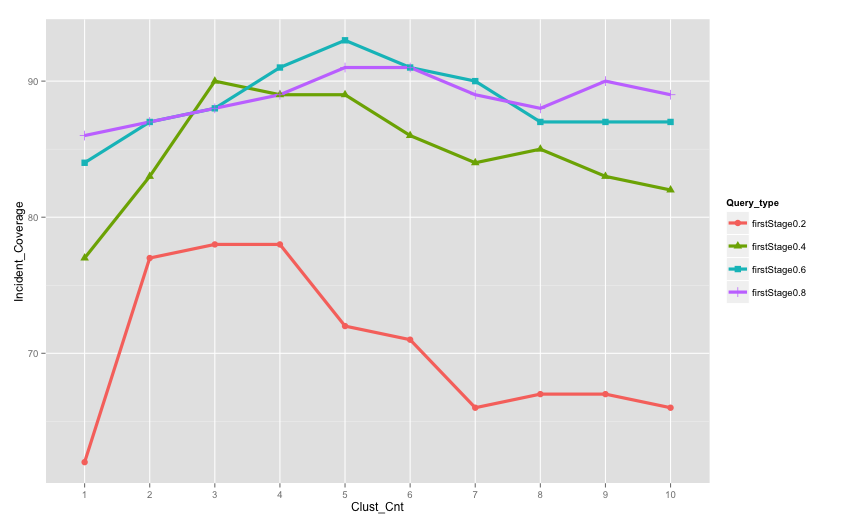
\includegraphics[width=9cm ,height=5.5cm]{figuresPng/Coverage_Result.png}
\caption{Incident coverage for different values of FSP. }
\label{fig: clustCoverage}
\end{figure}

\begin{figure}[!h]
\centering
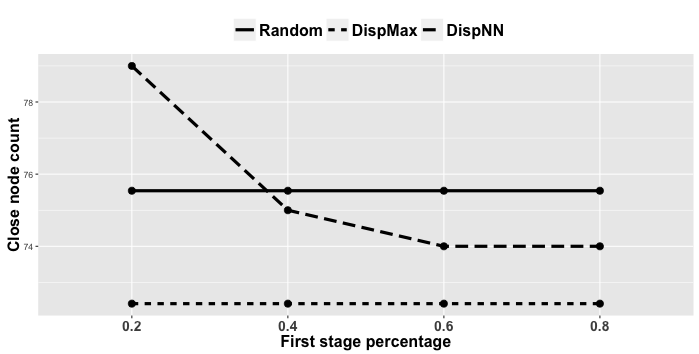
\includegraphics[width=9cm ,height=5.5cm]{figuresPng/Uni_ClosePeople_Count.png}
\caption{Close node count for different values of FSP. }
\label{fig:uniClosePeople}
\end{figure}
\begin{figure}[!h]
\centering
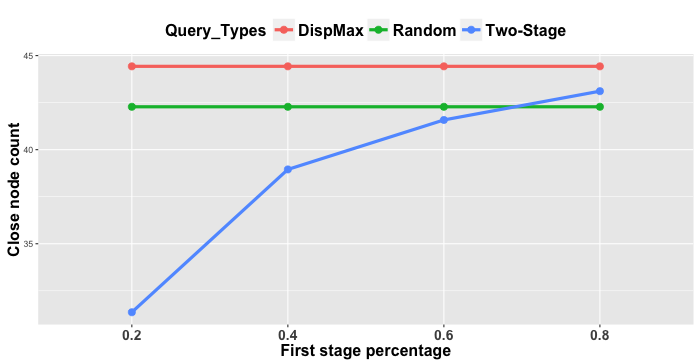
\includegraphics[width=9cm ,height=5.5cm]{figuresPng/Uni-Inc_Coverage.png}
\caption{Incident coverage for different values of FSP. }
\label{fig:uniIncdCove}
\end{figure}


\begin{figure}[!h]
\centering
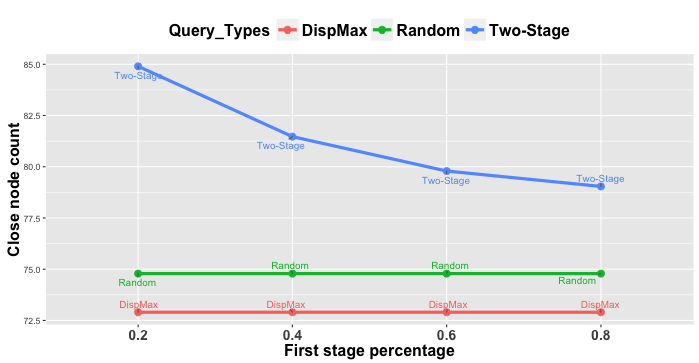
\includegraphics[width=9cm ,height=5.5cm]{figuresPng/LT-closePeople.png}
\caption{Close node count for different values of FSP in the case of a long tail distribution. }
\label{fig:LTClosePeople}
\end{figure}
\begin{figure}[!h]
\centering
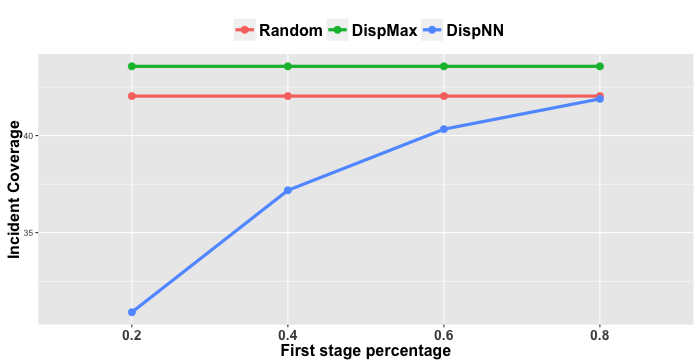
\includegraphics[width=9cm ,height=5.5cm]{figuresPng/LT-incidCov.png}
\caption{Incident coverage for different values of FSP in the case of a long tail distribution. }
\label{fig:LTIncdCove}
\end{figure}



\subsection{Case study: Hollaback harassment data set}
After applying DispNN to the previously mentioned three distributions (clustered, uniform and long-tail), we wish to examine the algorithm under real incident distributions. To do that, we test our querying algorithm on a global street harassment dataset provided by Hollaback~\cite{hollaback}.
\subsubsection{Data overview}
Hollaback is a non-profit movement powered by local activists in $92$ cities and $32$ countries to end street harassment. The Hollaback project collects data on street harassment events worldwide. Through the Hollaback phone app and the online platform, users can report stories of street harassment to share with the Hollaback community. This empowers victims to speak out about everyday harassment and spread the word about the prevalence of these events. In some communities, local governments are informed in real-time about street harassment so that there is a system-wide level of accountability. In addition, the Hollaback app uses GPS to record a data set that represents the locations of street harassment events as a means of improving the collective understanding of street harassment and how it can be prevented.  As of January $2016$, over $8000$ street harassment incidents have been recorded in their dataset since February $2011$.  It is on this data set that we wish to test DispNN.\par
\subsubsection{Analysis}
From the Hollaback dataset, we select cities for which we have enough harassment samples for statistical significance (i.e. more than 30 samples). We test the performance of Random selection, Dispersion maximization selection, and DispNN on six different cities: Paris, Brussels, Berlin, Baltimore, Buenos Aires and Istanbul. These cities were in the top ten cities with respect to the number of harassment reports in this dataset. In this paper, we show results for Paris, Brussels, and Istanbul. The results for Berlin, Baltimore, and Buenos Aires were consistent with the results shown in this paper. \par

As a first step, we must parse the Hollaback dataset such that incidents reports are grouped by city. To do so, we use bounding box coordinates. We then draw the border lines for the different cities and remove any outliers from our datasets. Figure~\ref{fig:citiesDistribution} shows the resulting distribution of events for the three-case study. The Paris dataset contains $197$ harassment incidents, while the Brussels dataset contains $154$ incidents covering a geographic area of $28.4$ $mi^2$. For Istanbul, we divide the coverage into two areas: $87$ reported incidents over an area of $138$ $mi^2$ on the left of the Bosporus Strait and $69$ $mi^2$ on the right. \par


\begin{table*}[t]
 \centering
 \begin{tabular}{ccc}
    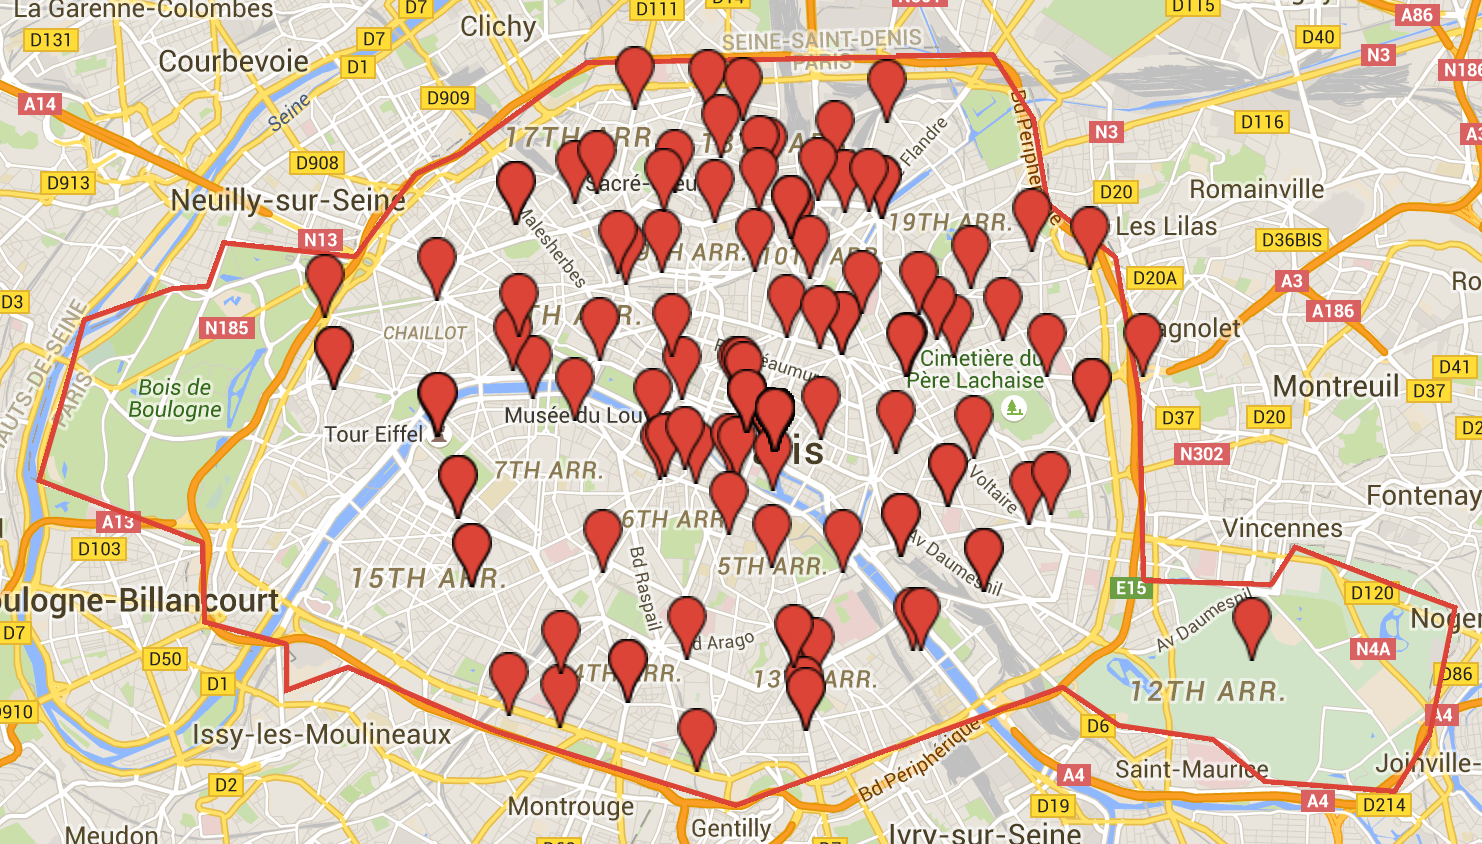
\includegraphics[width=0.33\textwidth, height=5cm]{figuresPng/Paris.png}&  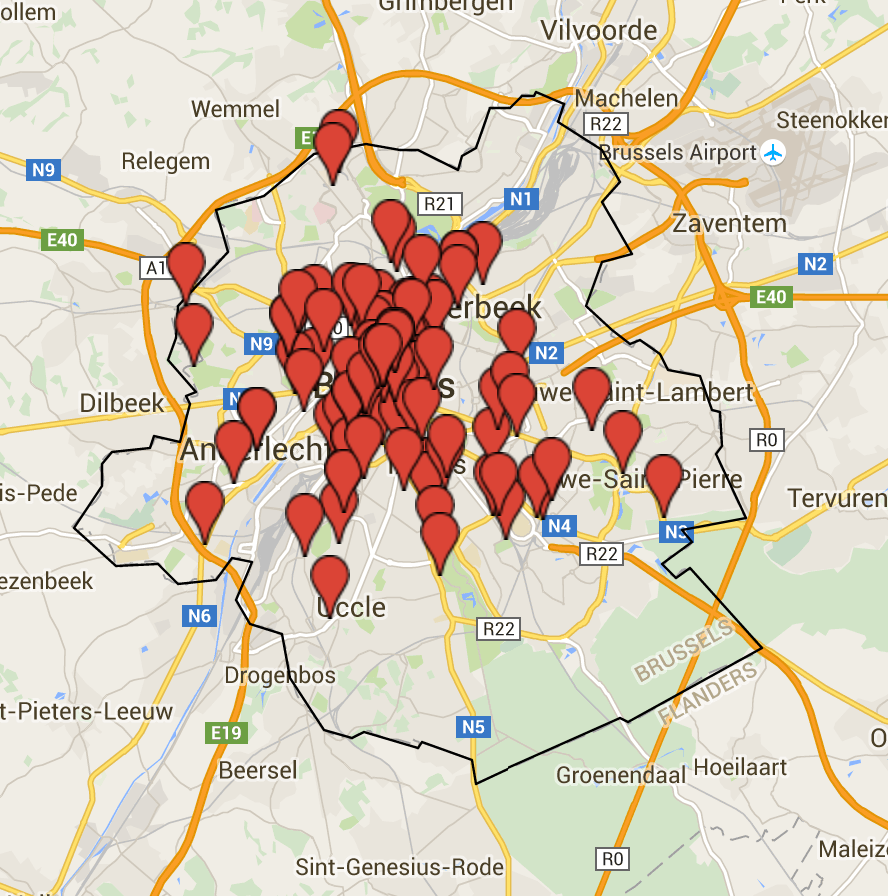
\includegraphics[width=0.33\textwidth, height=5cm]{figuresPng/Brussels.png} & 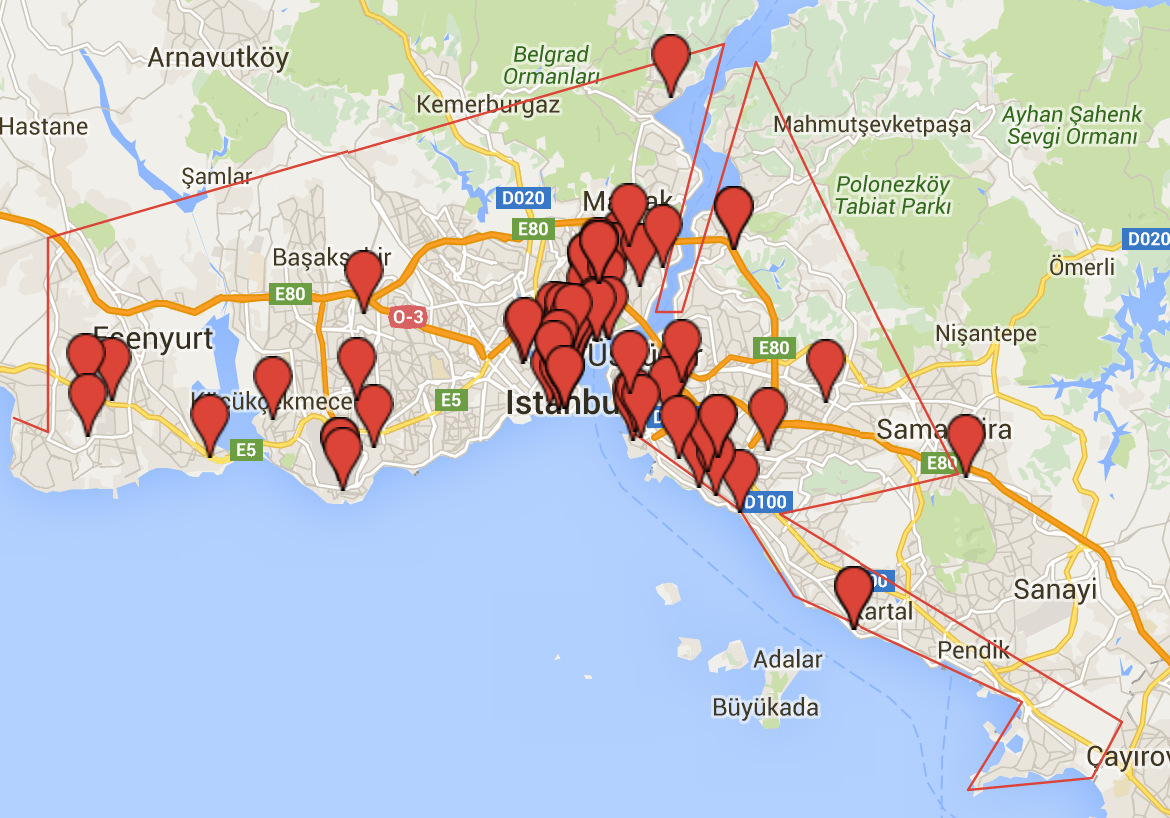
\includegraphics[width=0.33\textwidth, height=5cm]{figuresPng/Istanbul.png}\\
    (a) Paris & (b) Brussels & (c) Istanbul\\
 \end{tabular}
  \captionof{figure}{Distribution of harassment incidents across representative city datasets.}
\label{fig:citiesDistribution}
\end{table*}


%\begin{figure}[!h]
%\centering
%\subcaptionbox{ Paris: $197$ harassment incidents covering an area of $28.2$ $mi^2$. \label{fig: clust_20}}{%
%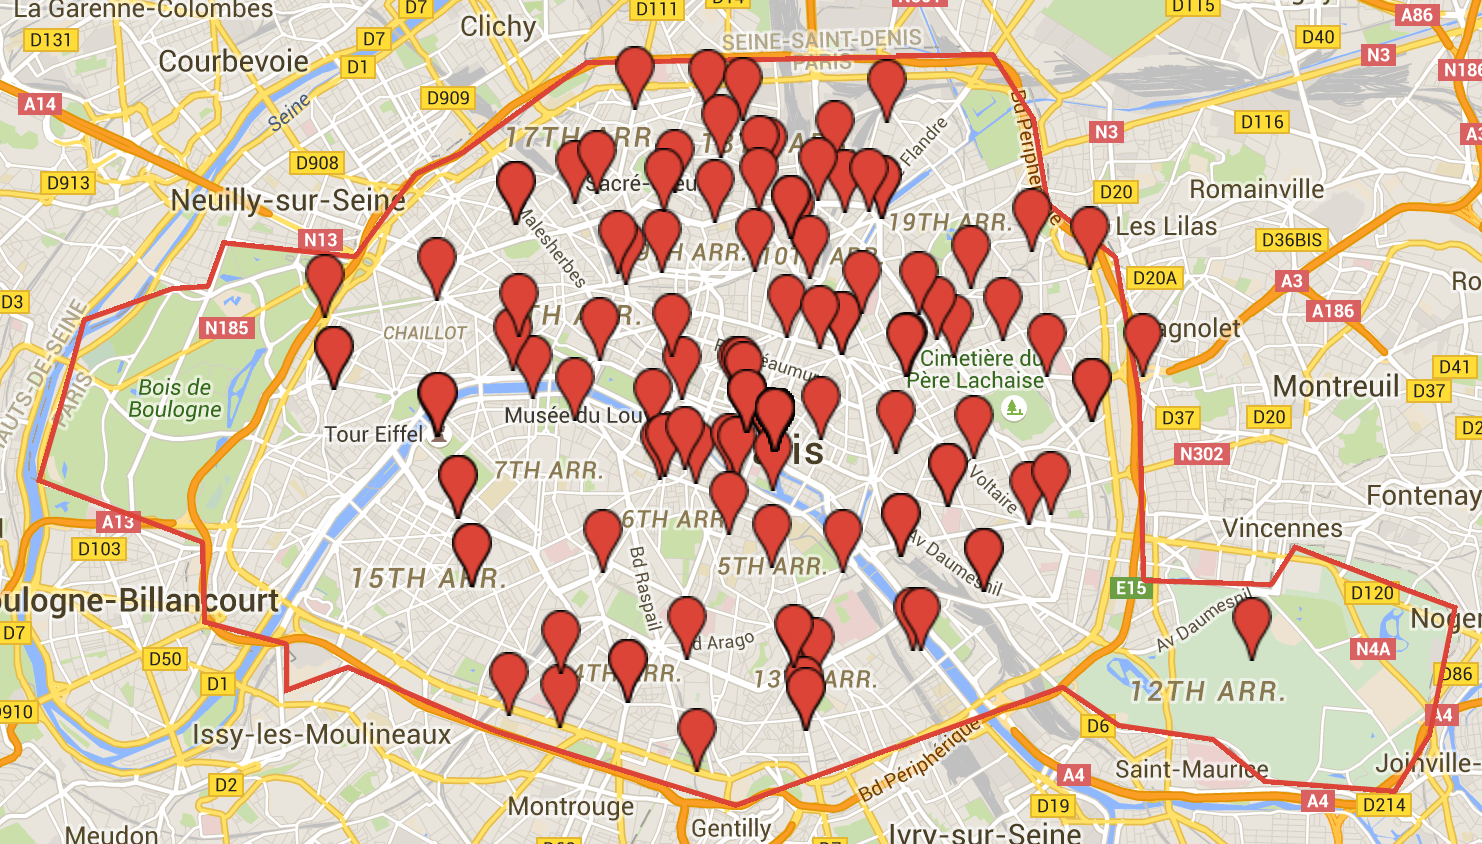
\includegraphics[width=8cm, height=5cm]{figuresPng/Paris.png}%
%}\par\medskip
%\subcaptionbox{Brussels: $154$ incidents covering an area of $28.4$ $mi^2$.\label{fig: clust_40}}{%
%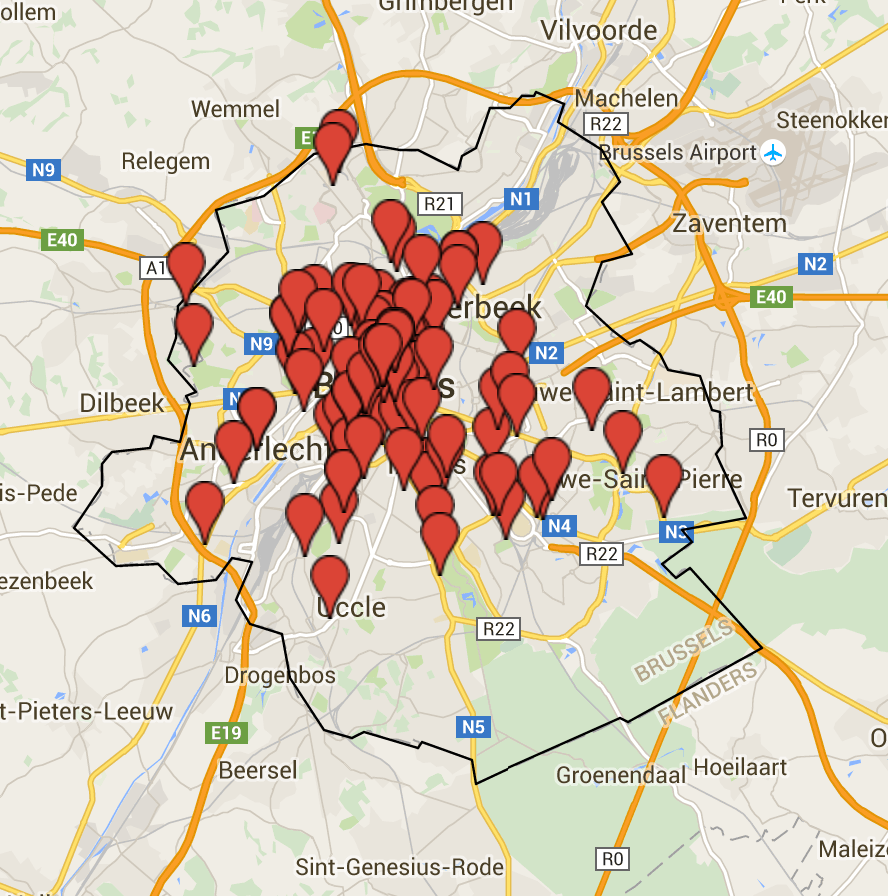
\includegraphics[width=8cm, height=5cm]{figuresPng/Brussels.png}%
%}\par\medskip   
%\subcaptionbox{ Istanbul: $87$ reported incidents covering an area of $138$ $mi^2$ on the left of the Bosporus Strait and $69$ $mi^2$ on the right.\label{fig: clust_60}}{%
%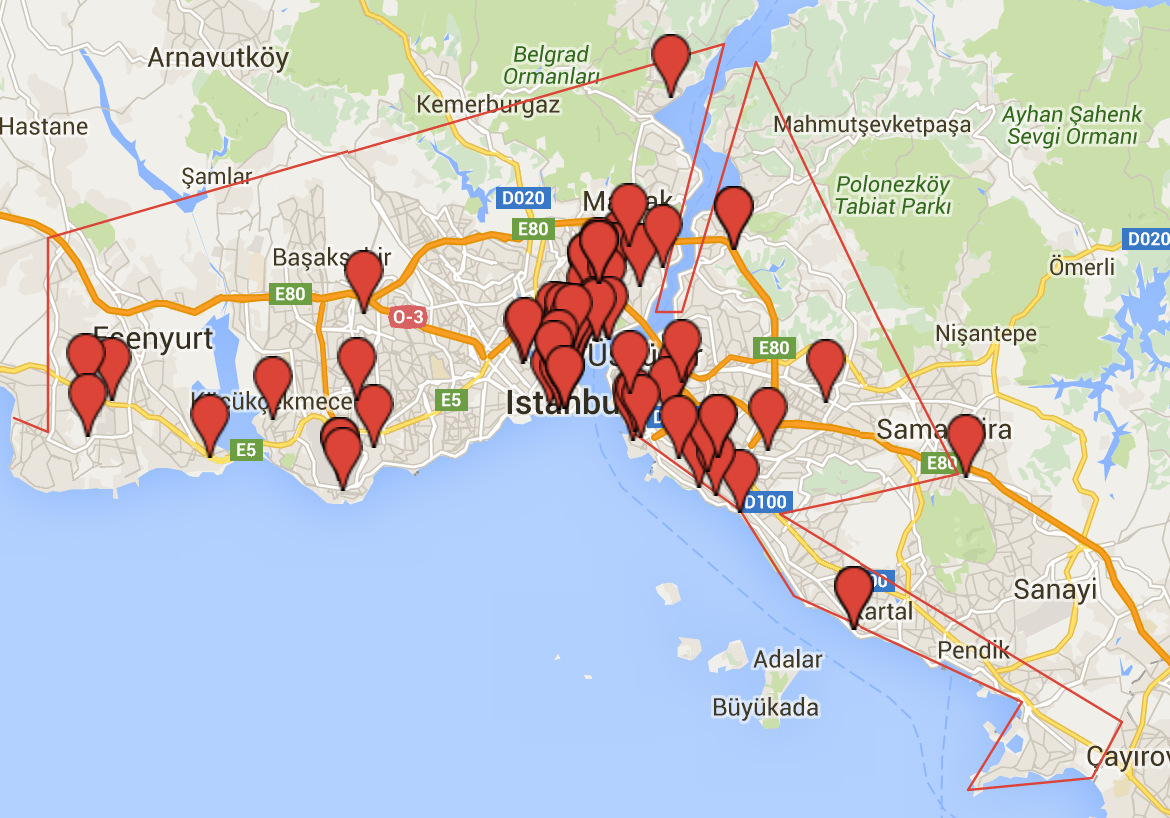
\includegraphics[width=8cm ,height=5cm]{figuresPng/Istanbul.png}%
%}
%\caption{Distribution of harassment incidents across representative city datasets.}
%\label{fig:citiesDistribution}
%\end{figure}


For each of the cities, we generate different variations of uniformly distributed crowds ($M = 100$) across the city. In this kind of analysis, the parameters, matrix dimension and incident count, are not generated by our analysis but rather taken from the dataset. In this case, we update the distance metric in Equation~\ref{eq:maxDisp} and use the Haversine formula to calculate the great-circle distance between two points as follows:
\begin{equation} \label{eq:maxDisp2}
d = 2R*atan2(\sqrt{a}, \sqrt{1-a})
\end{equation}
where $a$ is calculated as $ \sin ^2((\Delta \phi)/2 ) + \cos(\phi_1)\cos(\phi_2) * \sin ^2((\Delta \lambda)/2 )$, $\Delta \phi$ and $\Delta \lambda$ are calculated as the radian difference between the latitudes and longitudes, respectively, and $R$ is the Earth's radius (mean radius = 6,371km). We measure CNC and the Incident Coverage for all three querying approaches and plot the results in Figures~\ref{fig: hollaCloseCount} and~\ref{fig: hollaIncCoverage}, respectively. DispNN outperforms both the Random and Dispersion Maximization in terms of CNC for all three cities. In terms of incident coverage, Figure~\ref{fig: hollaIncCoverage} shows that dispersion maximization achieves maximum incident coverage. The figure also shows that DispNN can achieve this maximum by setting the first stage percentage to be $80\%$. Figures~\ref{fig: hollaCloseCount} and~\ref{fig: hollaIncCoverage} suggest that there is an inherent tradeoff between accuracy and coverage under constrained resources which we discuss in detail in later sections. The figures also suggest that DispNN with $FSP = 80\%$, can achieve a balance between accuracy and coverage.\par

\subsection{Stressing DispNN (k=1)}
After applying DispNN to different datasets, we are interested in checking which schemes were able to query nodes that were the first nearest neighbors to the incidents. This is beneficial, for example, when targeting first responders in an emergency scenario or in a spatial task distribution where you want to select the nearest neighbors to maximize spatial task assignment. This can be viewed as stressing the selection policies in order to determine which achieves a higher number of first nearest neighbors.\par

To study first nearest neighbors, we examine the Hollaback datasets for Paris, Brussels, and Istanbul. We examine the total CNC and for each incident, we determine whether we selected the first nearest neighbor in the queried users set. These results are shown in Table~\ref{table:NNParis}, where NN denotes nearest neighbors, CNC denotes close node count, and DispNN denotes the two-stage querying algorithm. For Paris, DispNN achieves a $9.5\%$ increase in performance on average in selecting nearest neighbors in comparison to dispersion maximization and a $19\%$ increase in comparison to random selection. For Brussels (Bruss), the performance gain is $14.2\%$ and $21.35\%$ in comparison to dispersion maximization and random selection, respectively. For Istanbul (Istan), the performance gains were $26.7\%$ and $36.5\%$. These results show that DispNN is able to locate more first nearest neighbors to incidents. This can be used to minimize the cost of traveling of users as a part of spatial task assignment. 

\section{Discussion}
\subsection{Tradeoff}
In the previous section, we examined the performance of the DispNN querying algorithm in a variety of incident and node/user configurations and we observed that as $FSP$ decreases, CNC tends to increase. We also observed that in this case the same node can be in the K nearest neighbors for multiple incidents. This means that the algorithm tends to select central nodes that are in proximity with other incidents. This is beneficial in cases where the centrality of nodes is important to the problem, e.g. minimizing trip costs to these incidents and maximizing task assignments. This observation can be used to diversify feedback to improve accuracy i.e., instead of relying on a small number of nodes close to the incidents, we have a greater sample that can contribute to the measurement.
On the other hand, as $FSP$ increases so does the probability of catching more incidents in the spatial environment, which is crucial in applications where coverage is important and where a false positive is less expensive than a false negative. This is due to the fact that more nodes are selected in the first stage and fewer nodes in the second stage. It is no surprise, under resource constrained conditions, there is a tradeoff between accuracy and coverage.

\subsection{Algorithm variants}
\subsubsection{Trust-based responses}
In our second stage of our algorithm, we select users based on the pivot nodes that provide a positive feedback in the first stage. To incorporate trust into the algorithm, trust-based algorithms can provide feedback about certain nodes and their feedback. If some of the nodes queried in the first stage of the algorithm were deemed trust unworthy, the second stage can be divided into two querying steps. The first step is the KNN for the trustworthy-nodes, and the second is determining dispersion maximization.
\subsubsection{Prior knowledge availability}
DispNN does not assume any knowledge about the distribution of events. Given some prior information about the distribution, the algorithm can be tailored to take the prior distribution into account. The idea is to divide the spatial area into bounding regions and for each region we give a specific weight that reflects the probability of occurrence in that bounding regions.
For example, Figure~\ref{fig: BaltimoreRegions} shows Baltimore divided into four bounding regions denoted as br1, br2, br3, and br4. Using the knowledge that br3 has more incidents than br2, which has more incidents than br1 and br4, a higher weight should be given to br3. In particular, $br3_w > br2_w> br4_w> br1_w$ where the subscript $w$ denotes the weight assigned to the bounding region. The next step would be to apply the algorithm on the different bounding regions taking into account the weights assigned when allocating resources as shown in Algorithm~\ref{TSBR}.


\begin{figure}[!h]
\centering
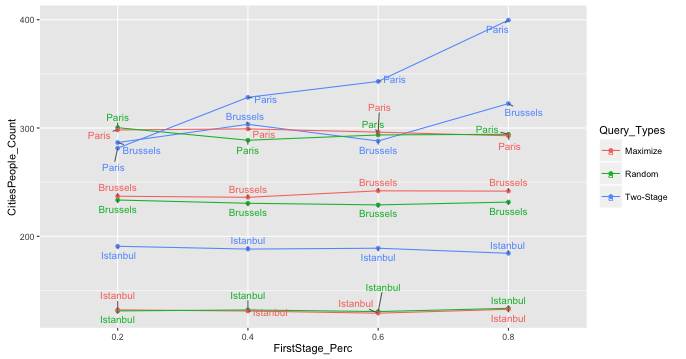
\includegraphics[width=9cm ,height=6cm]{figuresPng/hollaCloseCnt.png}
\caption{CNC for different values of FSP. }
\label{fig: hollaCloseCount}
\end{figure}
\begin{figure}[!h]
\centering
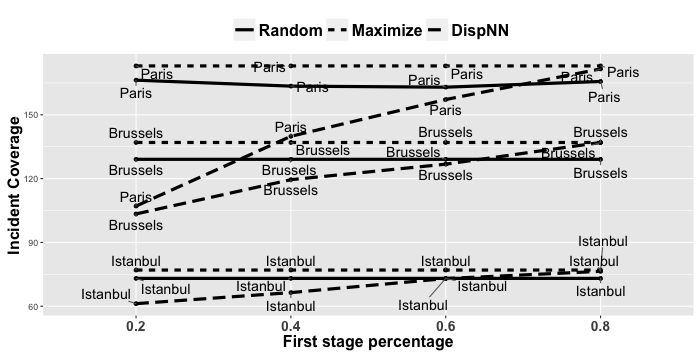
\includegraphics[width=9cm ,height=6cm]{figuresPng/citiesInc.png}
\caption{Incident coverage for different values of FSP. }
\label{fig: hollaIncCoverage}
\end{figure}


\begin{table}[!h]
\centering
\begin{tabulary}{0.5\textwidth}{|C|C|C|C|C|C|C|}
\hline
City & Random & DispMax & DispNN: $FSP = 20\%$ & DispNN: $FSP = 40\%$ & DispNN: $FSP = 60\%$ & DispNN: $FSP = 80\%$  \\ \hline
Paris-NN & $58$ & $63$  & $54$  & $69$ & $69$ & $84$  \\ \hline
Paris-CNC   & $300$ & $298$  & $281$  & $328$ & $343$ & $399$  \\ \hline
Bruss-NN & $48$ & $51$  & $55$  & $58$ & $55$ & $65$  \\ \hline
Bruss-CNC   & $233$ & $237$  & $286$  & $303$ & $288$ & $322$  \\ \hline
Istan-NN & $26$ & $28$  & $36$  & $37$ & $35$ & $36$  \\ \hline
Istan-CNC   & $131$ & $132$  & $190$  & $188$ & $188$ & $184$  \\ \hline
\end{tabulary}
\caption{First nearest neighbors (NN) count and CNC for Paris, Brussels, and Istanbul.}
\label{table:NNParis}
\end{table}




\begin{figure}[!h]
\centering
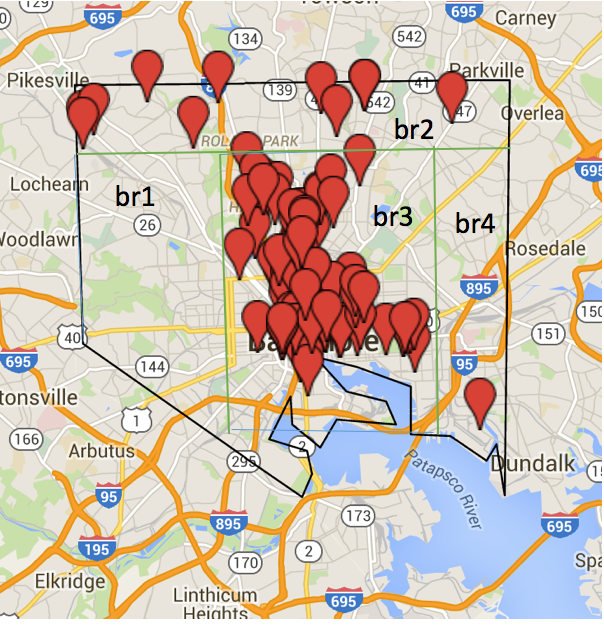
\includegraphics[width=9cm ,height=5.5cm]{figuresPng/BaltimoreBr.png}
\caption{Baltimore divided into bounding regions depending on prior knowledge of harassment occurrence.}
\label{fig: BaltimoreRegions}
\end{figure}


\begin{algorithm}
\caption{Bounding regions two-stage variation.}
\label{TSBR}
\begin{algorithmic}[1]
   \Function{selectUsersBRs }{$BRs[], w[], N, FSP$}
   \State selectedUsers = $\left\{\right\}$
    \State BRQuota = calculateQuota(BRs[], w[], N)
     \For{$br$ in BRs}
     \State brQuota = BRQuota(br)
   \State brUsers = selectUsersFromGrid(FSP, brQuota)
   \State brUsers.append(brUsers)
 \EndFor
\State return {selectedUsers}
\EndFunction
\end{algorithmic}
\end{algorithm}
\section{Conclusion}
This paper proposed DispNN: a two-stage spatial querying algorithm that attempts to probe nodes that are closer to the incidents in a $2D$ spatial environment. The algorithm maximizes the dispersion of location in the first stage and selects the K nearest neighbors in the second stage based on node feedback. The experimental evaluation confirms the applicability of proposed approach.
Important aspects that need to be taken into consideration include the sensing range and the sensing accuracy of the nodes. Nodes with accurate sensing and larger sensing ranges will provide more robustness to DispNN. Another important parameter that can impact the performance of the algorithm is the distribution of the available nodes in the spatial environment. To ensure an optimal performance, nodes should be placed uniformly in the environment if the incident distribution is not known or following an approximate distribution of the incidents. The node placement can be controlled for some sensors like traffic or agriculture sensors while in other cases it is hard to be controlled especially when human participation is involved. In that case, there are no guarantees that humans as sensors will be uniformly distributed across the spatial area under investigation. Another important factor when choosing the number of nodes to query is the granularity of the incidents. For instance, when using human as sensors, incidents such as disasters can likely be sensed/detected by numerous people in the range of the incident. On the other hand, incidents such as street harassment require the presence of the human at the same exact place of the incident; otherwise, the incident is unlikely to be detected.

\section{Acknowledgments}
The authors would like to thank Hollaback for sharing their collected dataset and taking the time to answer questions.
\bibliographystyle{abbrv}
{\footnotesize
\bibliography{sigproc}}  % sigproc.bib is the name of the Bibliography in this case
% You must have a proper ".bib" file
%  and remember to run:
% latex bibtex latex latex
% to resolve all references
%
% ACM needs 'a single self-contained file'!
%
%APPENDICES are optional
%\balancecolumns
\end{document}





